\section{Results}\label{sec:results}

\begin{table}[tbp]
\centering
\scriptsize
\setlength{\tabcolsep}{1.5pt}
\caption{Main results: test AUC and DPD, mean$\pm$sd over seeds. Best per column in bold; methods with mean AUC below 0.60 on a dataset (degenerate) are not bolded. $^\dagger$: Holm-adjusted Wilcoxon signed-rank $p<0.05$ against CLAMP, paired by seed.}
\label{tab:e1_main_compact}
\resizebox{\textwidth}{!}{%
\begin{tabular}{p{2.4cm} cc cc cc cc}
\toprule
 & \multicolumn{2}{c}{German} & \multicolumn{2}{c}{Bail} & \multicolumn{2}{c}{Credit} & \multicolumn{2}{c}{Pokec-z} \\
 & AUC & DPD & AUC & DPD & AUC & DPD & AUC & DPD \\
\midrule
\raggedright FedAvg-GAT & \textbf{0.76$\pm$0.05} & 0.110$\pm$0.058 & 0.80$\pm$0.04 & 0.019$\pm$0.011 & 0.77$\pm$0.01 & 0.078$\pm$0.010$^\dagger$ & 0.74$\pm$0.02 & 0.031$\pm$0.013 \\
\raggedright FairFed & 0.75$\pm$0.05 & 0.049$\pm$0.039 & \textbf{0.80$\pm$0.03} & 0.012$\pm$0.007 & 0.75$\pm$0.01 & 0.008$\pm$0.005 & 0.64$\pm$0.05$^\dagger$ & \textbf{0.004$\pm$0.003}$^\dagger$ \\
\raggedright F2GNN & 0.73$\pm$0.02 & \textbf{0.042$\pm$0.030} & 0.78$\pm$0.03 & 0.012$\pm$0.008 & 0.76$\pm$0.01 & \textbf{0.006$\pm$0.007} & 0.74$\pm$0.02 & 0.008$\pm$0.007$^\dagger$ \\
\raggedright FairGFL & 0.74$\pm$0.05 & 0.081$\pm$0.070 & 0.78$\pm$0.03 & 0.015$\pm$0.006 & 0.76$\pm$0.01 & 0.072$\pm$0.009$^\dagger$ & 0.66$\pm$0.02$^\dagger$ & 0.041$\pm$0.011 \\
\raggedright FedGraph-Fair & 0.66$\pm$0.09 & 0.080$\pm$0.051 & 0.76$\pm$0.03 & \textbf{0.010$\pm$0.007} & 0.75$\pm$0.01 & 0.075$\pm$0.014$^\dagger$ & 0.64$\pm$0.03$^\dagger$ & 0.039$\pm$0.013 \\
\raggedright FedFACT & 0.72$\pm$0.04 & 0.078$\pm$0.064 & 0.80$\pm$0.03 & 0.013$\pm$0.008 & 0.75$\pm$0.01 & 0.070$\pm$0.016$^\dagger$ & 0.63$\pm$0.04$^\dagger$ & 0.024$\pm$0.014 \\
\raggedright PUFFLE & 0.49$\pm$0.08$^\dagger$ & 0.011$\pm$0.007$^\dagger$ & 0.50$\pm$0.06$^\dagger$ & 0.003$\pm$0.003 & 0.46$\pm$0.13$^\dagger$ & 0.016$\pm$0.008 & 0.55$\pm$0.11$^\dagger$ & 0.008$\pm$0.009$^\dagger$ \\
\raggedright FedFDP & 0.53$\pm$0.09$^\dagger$ & 0.014$\pm$0.021 & 0.51$\pm$0.03$^\dagger$ & 0.004$\pm$0.003$^\dagger$ & 0.54$\pm$0.11$^\dagger$ & 0.017$\pm$0.009 & 0.64$\pm$0.11$^\dagger$ & 0.008$\pm$0.008$^\dagger$ \\
\raggedright FairGNN & 0.57$\pm$0.06$^\dagger$ & 0.111$\pm$0.082 & 0.56$\pm$0.09$^\dagger$ & 0.019$\pm$0.020 & 0.67$\pm$0.09$^\dagger$ & 0.100$\pm$0.055 & 0.54$\pm$0.08$^\dagger$ & 0.005$\pm$0.013 \\
\raggedright FairSIN & 0.72$\pm$0.05 & 0.092$\pm$0.062 & 0.79$\pm$0.03 & 0.025$\pm$0.008$^\dagger$ & 0.75$\pm$0.00 & 0.070$\pm$0.012$^\dagger$ & 0.66$\pm$0.05$^\dagger$ & 0.026$\pm$0.010 \\
\raggedright ClipMean (no controller, last iterate) & 0.73$\pm$0.06 & 0.088$\pm$0.069 & 0.78$\pm$0.03 & 0.016$\pm$0.009 & \textbf{0.77$\pm$0.01}$^\dagger$ & 0.071$\pm$0.009$^\dagger$ & 0.75$\pm$0.02 & 0.042$\pm$0.011$^\dagger$ \\
\raggedright CLAMP (last iterate) & 0.73$\pm$0.07 & 0.050$\pm$0.046 & 0.78$\pm$0.03 & 0.016$\pm$0.009 & 0.76$\pm$0.01 & 0.055$\pm$0.046 & 0.75$\pm$0.02 & 0.027$\pm$0.004 \\
\raggedright CLAMP-Select (no controller) & 0.73$\pm$0.06 & 0.077$\pm$0.066 & 0.78$\pm$0.03 & 0.016$\pm$0.009 & 0.77$\pm$0.01$^\dagger$ & 0.067$\pm$0.010$^\dagger$ & \textbf{0.75$\pm$0.02} & 0.041$\pm$0.010$^\dagger$ \\
\raggedright \textbf{CLAMP} & 0.72$\pm$0.06 & 0.058$\pm$0.044 & 0.78$\pm$0.03 & 0.016$\pm$0.009 & 0.76$\pm$0.01 & 0.018$\pm$0.015 & 0.75$\pm$0.02 & 0.026$\pm$0.004 \\
\raggedright CLAMP-GCN & 0.73$\pm$0.05 & 0.065$\pm$0.044 & 0.79$\pm$0.02 & 0.015$\pm$0.006 & 0.75$\pm$0.01 & 0.014$\pm$0.013 & 0.72$\pm$0.02$^\dagger$ & 0.028$\pm$0.006 \\
\bottomrule
\end{tabular}}
\vspace{4pt}
\resizebox{\textwidth}{!}{%
\begin{tabular}{p{2.4cm} cc cc cc cc}
\toprule
 & \multicolumn{2}{c}{Pokec-n} & \multicolumn{2}{c}{AMiner-S} & \multicolumn{2}{c}{NBA} & \multicolumn{2}{c}{Facebook} \\
 & AUC & DPD & AUC & DPD & AUC & DPD & AUC & DPD \\
\midrule
\raggedright FedAvg-GAT & 0.75$\pm$0.02 & 0.034$\pm$0.017 & 0.94$\pm$0.00 & 0.007$\pm$0.004$^\dagger$ & \textbf{0.81$\pm$0.06} & 0.099$\pm$0.059 & 0.77$\pm$0.05 & 0.078$\pm$0.048 \\
\raggedright FairFed & 0.62$\pm$0.06$^\dagger$ & \textbf{0.006$\pm$0.004}$^\dagger$ & 0.94$\pm$0.00 & 0.005$\pm$0.003 & 0.80$\pm$0.05 & 0.081$\pm$0.062 & 0.76$\pm$0.03 & \textbf{0.049$\pm$0.031} \\
\raggedright F2GNN & 0.74$\pm$0.03$^\dagger$ & 0.008$\pm$0.007$^\dagger$ & \textbf{0.94$\pm$0.01}$^\dagger$ & 0.005$\pm$0.004 & 0.78$\pm$0.13 & 0.109$\pm$0.072 & 0.76$\pm$0.05 & 0.069$\pm$0.040 \\
\raggedright FairGFL & 0.65$\pm$0.03$^\dagger$ & 0.044$\pm$0.007$^\dagger$ & 0.94$\pm$0.01 & 0.003$\pm$0.002 & 0.76$\pm$0.04 & 0.078$\pm$0.044 & 0.75$\pm$0.05 & 0.080$\pm$0.040 \\
\raggedright FedGraph-Fair & 0.59$\pm$0.05$^\dagger$ & 0.024$\pm$0.015 & 0.93$\pm$0.01$^\dagger$ & 0.003$\pm$0.003 & 0.77$\pm$0.10 & 0.084$\pm$0.043 & 0.74$\pm$0.05 & 0.094$\pm$0.037 \\
\raggedright FedFACT & 0.59$\pm$0.06$^\dagger$ & 0.012$\pm$0.011 & 0.92$\pm$0.01$^\dagger$ & 0.008$\pm$0.004 & 0.76$\pm$0.04 & 0.142$\pm$0.082 & 0.74$\pm$0.05 & 0.055$\pm$0.042 \\
\raggedright PUFFLE & 0.57$\pm$0.11$^\dagger$ & 0.010$\pm$0.006 & 0.49$\pm$0.03$^\dagger$ & 0.006$\pm$0.005 & 0.37$\pm$0.19 & 0.014$\pm$0.012 & 0.53$\pm$0.10$^\dagger$ & 0.009$\pm$0.006$^\dagger$ \\
\raggedright FedFDP & 0.66$\pm$0.08$^\dagger$ & 0.010$\pm$0.008 & 0.49$\pm$0.03$^\dagger$ & 0.006$\pm$0.004 & 0.39$\pm$0.20$^\dagger$ & 0.015$\pm$0.010$^\dagger$ & 0.54$\pm$0.08$^\dagger$ & 0.013$\pm$0.009 \\
\raggedright FairGNN & 0.50$\pm$0.00$^\dagger$ & 0.000$\pm$0.000$^\dagger$ & 0.63$\pm$0.08$^\dagger$ & 0.098$\pm$0.035$^\dagger$ & 0.77$\pm$0.08 & 0.097$\pm$0.044 & 0.51$\pm$0.05$^\dagger$ & 0.024$\pm$0.041 \\
\raggedright FairSIN & 0.64$\pm$0.06$^\dagger$ & 0.043$\pm$0.014 & 0.92$\pm$0.01$^\dagger$ & 0.005$\pm$0.003 & 0.73$\pm$0.08 & 0.087$\pm$0.059 & 0.74$\pm$0.05 & 0.070$\pm$0.033 \\
\raggedright ClipMean (no controller, last iterate) & 0.75$\pm$0.02 & 0.052$\pm$0.016$^\dagger$ & 0.94$\pm$0.01 & 0.005$\pm$0.004 & 0.78$\pm$0.08 & 0.093$\pm$0.068 & 0.77$\pm$0.06 & 0.086$\pm$0.043 \\
\raggedright CLAMP (last iterate) & 0.75$\pm$0.02 & 0.028$\pm$0.012 & 0.94$\pm$0.01 & 0.005$\pm$0.003 & 0.79$\pm$0.07 & 0.092$\pm$0.068 & \textbf{0.77$\pm$0.06} & 0.082$\pm$0.043 \\
\raggedright CLAMP-Select (no controller) & 0.75$\pm$0.02 & 0.052$\pm$0.015$^\dagger$ & 0.94$\pm$0.01 & 0.005$\pm$0.003 & 0.79$\pm$0.09 & \textbf{0.061$\pm$0.051} & 0.76$\pm$0.06 & 0.082$\pm$0.032 \\
\raggedright \textbf{CLAMP} & \textbf{0.76$\pm$0.02} & 0.028$\pm$0.012 & 0.94$\pm$0.01 & 0.004$\pm$0.004 & 0.80$\pm$0.08 & 0.076$\pm$0.054 & 0.76$\pm$0.06 & 0.069$\pm$0.034 \\
\raggedright CLAMP-GCN & 0.71$\pm$0.02$^\dagger$ & 0.027$\pm$0.008 & 0.94$\pm$0.00 & \textbf{0.002$\pm$0.002} & 0.78$\pm$0.07 & 0.077$\pm$0.044 & 0.76$\pm$0.04 & 0.078$\pm$0.030 \\
\bottomrule
\end{tabular}}
\end{table}


\subsection{Fairness and utility}\label{sec:main}

Table~\ref{tab:e1_main_compact} reports test AUC and $\dpd$ for all methods on the eight datasets; the full table with hard $\dpd$, $\eod$, backbones, the number of seeds within the budget and the record of Proposition~\ref{prop:cert} is in the appendix (Table~\ref{tab:e1_full}). We read it in three groups.

\paragraph{Where the budget binds}
On Credit, Pokec-z and Pokec-n the unconstrained clipped model (ClipMean) has a gap above the budget $\tau=0.03$ (0.071, 0.042 and 0.052). \clamp{} brings it to 0.018, 0.026 and 0.028, with AUC 0.76, 0.75 and 0.76 against 0.77, 0.75 and 0.75 for ClipMean; on Credit this AUC difference of 0.01 is statistically significant. The reduction is significant against ClipMean on all three graphs, but on the two Pokec graphs \clamp{}'s gap is not significantly lower than that of plain FedAvg-GAT (0.031 and 0.034), whose gap is already close to the budget. The test gap is at or below $\tau$ for 8, 9 and 5 of the 10 seeds; the remaining seeds exceed it on test data although the returned model met the budget on validation data, which is the validation--test generalisation gap that Proposition~\ref{prop:output} does not cover. These are soft gaps, the quantity the controller acts on. The hard gap at threshold 0.5 (appendix, Table~\ref{tab:e1_full}) is larger on Credit, 0.056 for \clamp{} against 0.104 for ClipMean and 0.116 for FedAvg-GAT, and there the baselines that use client information in the clear are close to \clamp{} (FairFed 0.048, F$^2$GNN 0.063); on the Pokec graphs the hard and soft gaps nearly coincide (\clamp{} 0.025 and 0.028). The baselines that read per-client fairness or group rates in the clear reach lower gaps: F$^2$GNN 0.006--0.008 at AUC 0.74--0.76, and FairFed 0.004--0.008, but at a large AUC cost on the Pokec graphs (0.62--0.64). \clamp{} is not designed to drive the gap to zero; it holds it at the budget the federation chooses, and Section~\ref{sec:tau} shows that lower budgets are reachable. FairGFL, FedGraph-Fair and FairSIN leave the gap close to that of FedAvg on Credit; FedFACT reduces it on the Pokec graphs (0.024 and 0.012) but at AUC 0.59--0.63. The two private methods, PUFFLE and FedFDP, have small gaps because they barely learn: with gradient noise at $\varepsilon=8$ their AUC lies between 0.37 and 0.66, and below 0.5 on several datasets (NBA, Credit, German), i.e.\ no better than chance. These two baselines are therefore not meaningful competitors at this privacy level in our implementation.

\paragraph{Where the budget does not bind}
On Bail and AMiner-S the unconstrained gap is already below $\tau$ (0.016 and 0.005), so the multiplier stays at zero, \clamp{} coincides with ClipMean, and all reasonable methods are within noise of each other.

\paragraph{Small graphs}
On German, NBA and Facebook (403 to 1{,}045 nodes) every method has a large seed-to-seed spread, and \clamp{} improves only modestly on ClipMean (German 0.088 to 0.058, NBA 0.093 to 0.076, Facebook 0.086 to 0.069), and in 2 to 4 of 10 runs no release round after the warm-up was feasible, so the output rule fell back to the last model. With a few dozen validation nodes per group and client, the validation gap is a poor proxy for the test gap; switching the statistics noise off does not change this (Section~\ref{sec:privacy}).

\paragraph{The output rule}
The rows labelled ``last iterate'' return the final model instead of the stored feasible one. On Credit this changes the mean gap from 0.018 to 0.055 and its standard deviation from 0.015 to 0.046: the signed penalty makes the gap oscillate around the budget, and the last iterate lands anywhere on the oscillation. With ten seeds this difference is not significant after Holm correction, and on the Pokec graphs the last iterate is as good as the selected model (0.027 and 0.028), so the rule matters mainly on Credit, where it reduces the spread. Selection without the controller (\clamp{}-Select, $\eta=0$) does not reproduce the effect: its gap is 0.067, 0.041 and 0.052 on Credit, Pokec-z and Pokec-n, close to ClipMean, and it finds an eligible feasible round in only 7, 2 and 1 of 10 runs. The controller creates feasible models and the output rule picks one. On Credit and the Pokec graphs the selected round is late (98--99 on average), so the returned model has been trained almost as long as the last one.

\subsection{Controllability of the fairness budget}\label{sec:tau}

\begin{figure}[t]
\centering
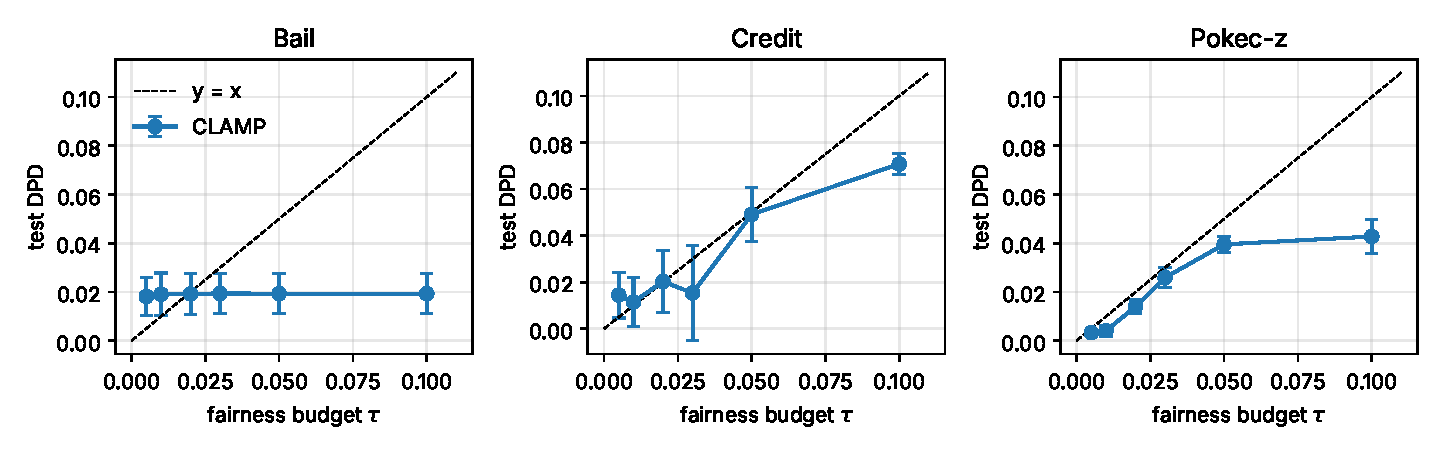
\includegraphics[width=0.6\linewidth]{figures/e2_tau_pareto}
\caption{Test $\dpd$ of \clamp{} against the budget $\tau$ (mean over five seeds; dashed: $\dpd=\tau$).}\label{fig:tau}
\end{figure}

Figure~\ref{fig:tau} varies $\tau$ from 0.005 to 0.1. On Pokec-z the test gap follows the budget (0.003, 0.004, 0.014, 0.026, 0.040 and 0.043 for the six values) while AUC stays at 0.74--0.75. On Credit the gap follows the budget down to about 0.012--0.020 and does not go lower: it is 0.012--0.020 for every $\tau\le0.03$, rises to 0.049 at $\tau=0.05$ and reaches the unconstrained 0.071 at $\tau=0.1$, and the tighter budgets cost about 0.01--0.02 AUC (0.77 to 0.75--0.76). On Bail the gap stays at 0.018--0.019 for every budget, with unchanged AUC: the controller does not reduce the test gap of this dataset. The budget therefore sets the operating point on two of the three datasets, within a range that depends on the dataset. At $\tau=0.005$, \clamp{} on Pokec-z reaches a lower gap than the best baseline (0.003 against 0.008 for F$^2$GNN) at a similar AUC (0.75 against 0.74).

\subsection{Byzantine updates}\label{sec:byz}
\begin{table}[tbp]
\centering
\scriptsize
\setlength{\tabcolsep}{2pt}
\caption{Update attacks on Bail: mean$\pm$sd over 3 seeds, $K=10$ clients. AUC (two decimals) and DPD (three decimals) at $f=0$ (no attack, None row only), $f=2$ and $f=4$ Byzantine clients. Best AUC per attack and $f$ in bold. $^\dagger$: median, trimmed mean and Krum inspect individual client updates and cannot run under secure aggregation. ClipMean: clipped mean with no fairness controller, last iterate.}
\label{tab:e3_bail}
\begin{tabular}{llcccccc}
\toprule
 & & \multicolumn{2}{c}{$f=0$} & \multicolumn{2}{c}{$f=2$} & \multicolumn{2}{c}{$f=4$} \\
 & & AUC & DPD & AUC & DPD & AUC & DPD \\
\midrule
\multirow{6}{*}{None} & FedAvg & \textbf{0.76$\pm$0.01} & 0.011$\pm$0.002 & -- & -- & -- & -- \\
 & Median$^\dagger$ & 0.73$\pm$0.01 & 0.007$\pm$0.000 & -- & -- & -- & -- \\
 & Trimmed mean$^\dagger$ & 0.75$\pm$0.02 & 0.013$\pm$0.002 & -- & -- & -- & -- \\
 & Krum$^\dagger$ & 0.72$\pm$0.02 & 0.003$\pm$0.001 & -- & -- & -- & -- \\
 & CLAMP & 0.75$\pm$0.02 & 0.011$\pm$0.002 & -- & -- & -- & -- \\
 & ClipMean & 0.75$\pm$0.02 & 0.009$\pm$0.003 & -- & -- & -- & -- \\
\midrule
\multirow{6}{*}{Sign-flip} & FedAvg & -- & -- & 0.38$\pm$0.03 & 0.020$\pm$0.012 & 0.39$\pm$0.03 & 0.032$\pm$0.002 \\
 & Median$^\dagger$ & -- & -- & 0.68$\pm$0.04 & 0.011$\pm$0.006 & 0.63$\pm$0.04 & 0.012$\pm$0.006 \\
 & Trimmed mean$^\dagger$ & -- & -- & \textbf{0.70$\pm$0.04} & 0.012$\pm$0.001 & 0.65$\pm$0.03 & 0.023$\pm$0.011 \\
 & Krum$^\dagger$ & -- & -- & 0.70$\pm$0.03 & 0.007$\pm$0.004 & \textbf{0.71$\pm$0.02} & 0.010$\pm$0.004 \\
 & CLAMP & -- & -- & 0.69$\pm$0.04 & 0.010$\pm$0.009 & 0.66$\pm$0.03 & 0.014$\pm$0.009 \\
 & ClipMean & -- & -- & 0.69$\pm$0.04 & 0.010$\pm$0.009 & 0.66$\pm$0.04 & 0.013$\pm$0.010 \\
\midrule
\multirow{6}{*}{Scaling} & FedAvg & -- & -- & 0.49$\pm$0.04 & 0.011$\pm$0.005 & 0.54$\pm$0.07 & 0.002$\pm$0.001 \\
 & Median$^\dagger$ & -- & -- & 0.73$\pm$0.03 & 0.010$\pm$0.003 & 0.73$\pm$0.02 & 0.005$\pm$0.005 \\
 & Trimmed mean$^\dagger$ & -- & -- & \textbf{0.75$\pm$0.01} & 0.012$\pm$0.007 & \textbf{0.75$\pm$0.01} & 0.008$\pm$0.002 \\
 & Krum$^\dagger$ & -- & -- & 0.71$\pm$0.02 & 0.006$\pm$0.005 & 0.71$\pm$0.02 & 0.010$\pm$0.004 \\
 & CLAMP & -- & -- & 0.75$\pm$0.02 & 0.010$\pm$0.002 & 0.75$\pm$0.02 & 0.011$\pm$0.002 \\
 & ClipMean & -- & -- & 0.75$\pm$0.02 & 0.009$\pm$0.003 & 0.75$\pm$0.02 & 0.009$\pm$0.003 \\
\midrule
\multirow{6}{*}{ALIE} & FedAvg & -- & -- & \textbf{0.73$\pm$0.03} & 0.012$\pm$0.001 & \textbf{0.72$\pm$0.02} & 0.008$\pm$0.002 \\
 & Median$^\dagger$ & -- & -- & 0.72$\pm$0.03 & 0.007$\pm$0.003 & 0.70$\pm$0.03 & 0.002$\pm$0.002 \\
 & Trimmed mean$^\dagger$ & -- & -- & 0.73$\pm$0.03 & 0.009$\pm$0.002 & 0.70$\pm$0.03 & 0.002$\pm$0.001 \\
 & Krum$^\dagger$ & -- & -- & 0.73$\pm$0.03 & 0.008$\pm$0.001 & 0.70$\pm$0.03 & 0.002$\pm$0.002 \\
 & CLAMP & -- & -- & 0.72$\pm$0.03 & 0.008$\pm$0.000 & 0.72$\pm$0.03 & 0.008$\pm$0.002 \\
 & ClipMean & -- & -- & 0.72$\pm$0.03 & 0.007$\pm$0.002 & 0.72$\pm$0.03 & 0.006$\pm$0.001 \\
\midrule
\multirow{6}{*}{IPM} & FedAvg & -- & -- & 0.72$\pm$0.02 & 0.010$\pm$0.001 & \textbf{0.71$\pm$0.02} & 0.009$\pm$0.002 \\
 & Median$^\dagger$ & -- & -- & 0.71$\pm$0.03 & 0.005$\pm$0.002 & 0.63$\pm$0.05 & 0.007$\pm$0.002 \\
 & Trimmed mean$^\dagger$ & -- & -- & \textbf{0.72$\pm$0.03} & 0.009$\pm$0.001 & 0.67$\pm$0.03 & 0.005$\pm$0.002 \\
 & Krum$^\dagger$ & -- & -- & 0.47$\pm$0.02 & 0.005$\pm$0.005 & 0.38$\pm$0.03 & 0.022$\pm$0.006 \\
 & CLAMP & -- & -- & 0.72$\pm$0.03 & 0.007$\pm$0.001 & 0.71$\pm$0.02 & 0.005$\pm$0.002 \\
 & ClipMean & -- & -- & 0.72$\pm$0.03 & 0.006$\pm$0.002 & 0.71$\pm$0.02 & 0.005$\pm$0.001 \\
\midrule
\multirow{6}{*}{Fairness-poison} & FedAvg & -- & -- & 0.72$\pm$0.02 & 0.014$\pm$0.011 & 0.70$\pm$0.03 & 0.021$\pm$0.008 \\
 & Median$^\dagger$ & -- & -- & 0.72$\pm$0.03 & 0.009$\pm$0.006 & 0.71$\pm$0.04 & 0.013$\pm$0.008 \\
 & Trimmed mean$^\dagger$ & -- & -- & \textbf{0.73$\pm$0.03} & 0.010$\pm$0.009 & \textbf{0.72$\pm$0.02} & 0.014$\pm$0.003 \\
 & Krum$^\dagger$ & -- & -- & 0.71$\pm$0.01 & 0.009$\pm$0.001 & 0.71$\pm$0.00 & 0.009$\pm$0.007 \\
 & CLAMP & -- & -- & 0.72$\pm$0.03 & 0.011$\pm$0.008 & 0.72$\pm$0.02 & 0.014$\pm$0.001 \\
 & ClipMean & -- & -- & 0.72$\pm$0.03 & 0.010$\pm$0.008 & 0.71$\pm$0.02 & 0.023$\pm$0.009 \\
\bottomrule
\end{tabular}
\end{table}

\begin{table}[tbp]
\centering
\scriptsize
\setlength{\tabcolsep}{2pt}
\caption{Update attacks on Pokec-z: mean$\pm$sd over 3 seeds, $K=10$ clients. AUC (two decimals) and DPD (three decimals) at $f=0$ (no attack, None row only), $f=2$ and $f=4$ Byzantine clients. Best AUC per attack and $f$ in bold. $^\dagger$: median, trimmed mean and Krum inspect individual client updates and cannot run under secure aggregation. ClipMean: clipped mean with no fairness controller, last iterate.}
\label{tab:e3_pokec}
\begin{tabular}{llcccccc}
\toprule
 & & \multicolumn{2}{c}{$f=0$} & \multicolumn{2}{c}{$f=2$} & \multicolumn{2}{c}{$f=4$} \\
 & & AUC & DPD & AUC & DPD & AUC & DPD \\
\midrule
\multirow{6}{*}{None} & FedAvg & 0.75$\pm$0.01 & 0.035$\pm$0.010 & -- & -- & -- & -- \\
 & Median$^\dagger$ & 0.75$\pm$0.01 & 0.033$\pm$0.009 & -- & -- & -- & -- \\
 & Trimmed mean$^\dagger$ & 0.74$\pm$0.01 & 0.035$\pm$0.007 & -- & -- & -- & -- \\
 & Krum$^\dagger$ & 0.74$\pm$0.02 & 0.033$\pm$0.014 & -- & -- & -- & -- \\
 & CLAMP & \textbf{0.76$\pm$0.00} & 0.028$\pm$0.016 & -- & -- & -- & -- \\
 & ClipMean & 0.76$\pm$0.00 & 0.045$\pm$0.007 & -- & -- & -- & -- \\
\midrule
\multirow{6}{*}{Sign-flip} & FedAvg & -- & -- & 0.50$\pm$0.01 & 0.001$\pm$0.002 & 0.49$\pm$0.01 & 0.001$\pm$0.001 \\
 & Median$^\dagger$ & -- & -- & 0.74$\pm$0.01 & 0.034$\pm$0.010 & 0.65$\pm$0.06 & 0.015$\pm$0.009 \\
 & Trimmed mean$^\dagger$ & -- & -- & 0.73$\pm$0.03 & 0.019$\pm$0.015 & 0.68$\pm$0.08 & 0.022$\pm$0.022 \\
 & Krum$^\dagger$ & -- & -- & 0.74$\pm$0.02 & 0.029$\pm$0.007 & \textbf{0.72$\pm$0.01} & 0.033$\pm$0.009 \\
 & CLAMP & -- & -- & 0.75$\pm$0.02 & 0.022$\pm$0.013 & 0.71$\pm$0.05 & 0.017$\pm$0.013 \\
 & ClipMean & -- & -- & \textbf{0.75$\pm$0.02} & 0.032$\pm$0.014 & 0.71$\pm$0.05 & 0.016$\pm$0.011 \\
\midrule
\multirow{6}{*}{Scaling} & FedAvg & -- & -- & 0.64$\pm$0.01 & 0.029$\pm$0.025 & 0.57$\pm$0.13 & 0.031$\pm$0.025 \\
 & Median$^\dagger$ & -- & -- & 0.76$\pm$0.01 & 0.033$\pm$0.003 & 0.76$\pm$0.01 & 0.036$\pm$0.014 \\
 & Trimmed mean$^\dagger$ & -- & -- & 0.71$\pm$0.01 & 0.030$\pm$0.007 & 0.74$\pm$0.02 & 0.038$\pm$0.011 \\
 & Krum$^\dagger$ & -- & -- & 0.73$\pm$0.01 & 0.034$\pm$0.004 & 0.71$\pm$0.03 & 0.031$\pm$0.003 \\
 & CLAMP & -- & -- & 0.76$\pm$0.00 & 0.027$\pm$0.017 & 0.76$\pm$0.00 & 0.028$\pm$0.016 \\
 & ClipMean & -- & -- & \textbf{0.76$\pm$0.00} & 0.045$\pm$0.007 & \textbf{0.76$\pm$0.00} & 0.045$\pm$0.007 \\
\midrule
\multirow{6}{*}{ALIE} & FedAvg & -- & -- & 0.74$\pm$0.00 & 0.032$\pm$0.012 & \textbf{0.75$\pm$0.02} & 0.031$\pm$0.009 \\
 & Median$^\dagger$ & -- & -- & 0.74$\pm$0.01 & 0.032$\pm$0.013 & 0.72$\pm$0.01 & 0.029$\pm$0.010 \\
 & Trimmed mean$^\dagger$ & -- & -- & 0.72$\pm$0.01 & 0.035$\pm$0.015 & 0.73$\pm$0.02 & 0.024$\pm$0.008 \\
 & Krum$^\dagger$ & -- & -- & 0.74$\pm$0.01 & 0.034$\pm$0.010 & 0.74$\pm$0.01 & 0.017$\pm$0.012 \\
 & CLAMP & -- & -- & \textbf{0.76$\pm$0.01} & 0.024$\pm$0.018 & 0.75$\pm$0.01 & 0.027$\pm$0.008 \\
 & ClipMean & -- & -- & 0.75$\pm$0.00 & 0.039$\pm$0.010 & 0.75$\pm$0.01 & 0.038$\pm$0.007 \\
\midrule
\multirow{6}{*}{IPM} & FedAvg & -- & -- & 0.76$\pm$0.01 & 0.039$\pm$0.010 & 0.75$\pm$0.01 & 0.035$\pm$0.004 \\
 & Median$^\dagger$ & -- & -- & 0.76$\pm$0.00 & 0.040$\pm$0.011 & 0.75$\pm$0.03 & 0.014$\pm$0.008 \\
 & Trimmed mean$^\dagger$ & -- & -- & 0.75$\pm$0.00 & 0.039$\pm$0.010 & \textbf{0.77$\pm$0.01} & 0.027$\pm$0.004 \\
 & Krum$^\dagger$ & -- & -- & 0.40$\pm$0.13 & 0.009$\pm$0.011 & 0.37$\pm$0.06 & 0.009$\pm$0.010 \\
 & CLAMP & -- & -- & 0.77$\pm$0.00 & 0.028$\pm$0.014 & 0.76$\pm$0.02 & 0.026$\pm$0.005 \\
 & ClipMean & -- & -- & \textbf{0.77$\pm$0.00} & 0.046$\pm$0.009 & 0.76$\pm$0.02 & 0.026$\pm$0.005 \\
\midrule
\multirow{6}{*}{Fairness-poison} & FedAvg & -- & -- & 0.71$\pm$0.03 & 0.124$\pm$0.027 & 0.69$\pm$0.03 & 0.137$\pm$0.068 \\
 & Median$^\dagger$ & -- & -- & 0.72$\pm$0.00 & 0.108$\pm$0.025 & 0.72$\pm$0.02 & 0.111$\pm$0.031 \\
 & Trimmed mean$^\dagger$ & -- & -- & 0.70$\pm$0.01 & 0.146$\pm$0.036 & 0.71$\pm$0.01 & 0.201$\pm$0.061 \\
 & Krum$^\dagger$ & -- & -- & 0.72$\pm$0.02 & 0.034$\pm$0.011 & 0.71$\pm$0.04 & 0.086$\pm$0.099 \\
 & CLAMP & -- & -- & 0.72$\pm$0.02 & 0.037$\pm$0.006 & 0.71$\pm$0.03 & 0.047$\pm$0.042 \\
 & ClipMean & -- & -- & \textbf{0.75$\pm$0.00} & 0.137$\pm$0.017 & \textbf{0.73$\pm$0.00} & 0.125$\pm$0.103 \\
\bottomrule
\end{tabular}
\end{table}

Tables~\ref{tab:e3_bail} and~\ref{tab:e3_pokec} report AUC and $\dpd$ under five update attacks with $f=2$ and $f=4$ of $K=10$ clients (three seeds; all $f$ with standard deviations in Table~\ref{tab:e3_full}). The rules marked $^\dagger$ need individual updates and cannot run under secure aggregation; they are reference points, not alternatives for the setting we study.

\paragraph{Model utility}
Plain FedAvg collapses under sign flipping (Pokec-z AUC 0.49--0.50 for $f\ge2$, Bail 0.37--0.39) and degrades under scaling. ClipMean, i.e.\ clipping without the controller, has the same AUC as \clamp{} under every attack, so the utility of \clamp{} under update attacks comes from clipping. Clipping protects completely against scaling (AUC 0.76 on Pokec-z and 0.75 on Bail for every $f$), because a scaled update is cut to norm $C$ like any other. Against sign flipping, \clamp{} degrades gradually: Pokec-z 0.76 to 0.71 and Bail 0.73 to 0.66 from $f=1$ to $f=4$. This is similar to the coordinate median and the trimmed mean (Pokec-z 0.65 and 0.68 at $f=4$) and worse than Krum on Bail (0.71). Against ALIE and IPM, which keep the malicious updates within the spread of honest ones, \clamp{} loses at most 0.04 AUC. The median and the trimmed mean lose more on Bail under IPM at $f=4$ (0.63 and 0.67), and Krum fails under IPM (Pokec-z AUC 0.35--0.40 for $f\ge2$). With three seeds these comparisons are indicative only. A norm bound limits how far any attack can move the model, but it does not filter attacks that stay within the bound, so we claim that \clamp{} is comparable to, not better than, robust rules that see individual updates.

\paragraph{Fairness under attack}
The fairness-poisoning attack trains Byzantine clients to increase the gap. On Pokec-z it raises the gap of FedAvg from 0.035 to 0.124--0.137 for $f\ge2$. The robust rules do not stop it, because the poisoned updates are not outliers: the median reaches 0.108--0.148 and the trimmed mean 0.146--0.201. Clipping alone does not stop it either: ClipMean reaches 0.137 at $f=2$ and 0.125 at $f=4$. Krum holds the gap at 0.034--0.035 up to $f=3$ and reaches 0.086 at $f=4$. \clamp{} keeps it at 0.037 at $f=2$ and 0.047 $\pm$ 0.042 at $f=4$, above the budget but far below the rules without fairness control. The difference to ClipMean, which shares everything except the controller, isolates the controller as the cause: the honest clients' statistics reveal the growing gap, and the multiplier counteracts it. On Bail, whose gap is small, the attack raises ClipMean only to 0.023 at $f=4$, and \clamp{} stays at 0.014. When an adversary manipulates the model's fairness through its updates rather than through the statistics, the honest majority's statistics are enough to counter it, in contrast to the statistics attack below.

\subsection{Falsified statistics}\label{sec:statattack}

\begin{table}[tbp]
\centering
\footnotesize
\caption{Statistics attacks. $|\widehat{D}-D^H|_{\max}$: largest deviation of the server's estimate from the honest-only gap over the release rounds; Bound: largest Theorem 3 bound (honest-mass term plus statistics-noise term, $\beta=0.05$) over the release rounds; Viol.: release rounds with the deviation above the bound. Each row covers 300 release rounds (3 seeds of 100 rounds); $f$ is the number of falsifying clients out of $K=10$. The bound uses the public cap (the cap the attack ran with), so it is computable without any group-level count. AUC and DPD: mean$\pm$sd over seeds.}
\label{tab:e4_stat_attacks}
\begin{tabular}{llcccccc}
\toprule
Dataset & Attack & $f$ & $|\widehat{D}-D^H|_{\max}$ & Bound & Viol. & AUC & DPD \\
\midrule
Bail & none & 0 & 0.017 & 0.070 & 0 & 0.75$\pm$0.02 & 0.009$\pm$0.003 \\
Bail & swap & 1 & 0.012 & 0.769 & 0 & 0.74$\pm$0.02 & 0.009$\pm$0.003 \\
Bail & swap & 2 & 0.011 & 1.273 & 0 & 0.74$\pm$0.02 & 0.009$\pm$0.003 \\
Bail & swap & 3 & 0.009 & 1.526 & 0 & 0.74$\pm$0.02 & 0.010$\pm$0.003 \\
Bail & swap & 4 & 0.007 & 1.688 & 0 & 0.74$\pm$0.02 & 0.009$\pm$0.003 \\
Bail & mid & 1 & 0.012 & 0.769 & 0 & 0.75$\pm$0.02 & 0.009$\pm$0.003 \\
Bail & mid & 2 & 0.010 & 1.273 & 0 & 0.75$\pm$0.02 & 0.009$\pm$0.003 \\
Bail & mid & 3 & 0.009 & 1.526 & 0 & 0.74$\pm$0.02 & 0.010$\pm$0.003 \\
Bail & mid & 4 & 0.007 & 1.688 & 0 & 0.75$\pm$0.02 & 0.009$\pm$0.003 \\
Pokec-z & none & 0 & 0.006 & 0.021 & 0 & 0.76$\pm$0.00 & 0.028$\pm$0.016 \\
Pokec-z & swap & 1 & 0.035 & 0.738 & 0 & 0.76$\pm$0.00 & 0.045$\pm$0.008 \\
Pokec-z & swap & 2 & 0.037 & 1.219 & 0 & 0.77$\pm$0.00 & 0.046$\pm$0.008 \\
Pokec-z & swap & 3 & 0.029 & 1.448 & 0 & 0.77$\pm$0.00 & 0.045$\pm$0.008 \\
Pokec-z & swap & 4 & 0.024 & 1.592 & 0 & 0.77$\pm$0.01 & 0.045$\pm$0.008 \\
Pokec-z & mid & 1 & 0.020 & 0.738 & 0 & 0.76$\pm$0.00 & 0.045$\pm$0.008 \\
Pokec-z & mid & 2 & 0.030 & 1.219 & 0 & 0.76$\pm$0.00 & 0.045$\pm$0.008 \\
Pokec-z & mid & 3 & 0.035 & 1.448 & 0 & 0.76$\pm$0.00 & 0.045$\pm$0.008 \\
Pokec-z & mid & 4 & 0.040 & 1.592 & 0 & 0.76$\pm$0.00 & 0.045$\pm$0.008 \\
Credit & none & 0 & 0.051 & 0.141 & 0 & 0.76$\pm$0.01 & 0.011$\pm$0.004 \\
Credit & swap & 1 & 0.066 & 1.115 & 0 & 0.76$\pm$0.01 & 0.065$\pm$0.008 \\
Credit & swap & 2 & 0.057 & 1.421 & 0 & 0.76$\pm$0.01 & 0.065$\pm$0.008 \\
Credit & swap & 3 & 0.045 & 1.617 & 0 & 0.76$\pm$0.01 & 0.064$\pm$0.008 \\
Credit & swap & 4 & 0.110 & 1.830 & 0 & 0.71$\pm$0.09 & 0.199$\pm$0.228 \\
Credit & mid & 1 & 0.057 & 1.115 & 0 & 0.76$\pm$0.00 & 0.064$\pm$0.008 \\
Credit & mid & 2 & 0.059 & 1.421 & 0 & 0.76$\pm$0.01 & 0.065$\pm$0.008 \\
Credit & mid & 3 & 0.062 & 1.617 & 0 & 0.76$\pm$0.01 & 0.064$\pm$0.008 \\
Credit & mid & 4 & 0.063 & 1.830 & 0 & 0.76$\pm$0.01 & 0.064$\pm$0.008 \\
\bottomrule
\end{tabular}
\end{table}


Table~\ref{tab:e4_stat_attacks} lets $b\in\{1,\dots,4\}$ of $K=10$ clients falsify their statistics. First, the bound of Theorem~\ref{thm:stats} is not informative here. Computed with the public cap, it ranges from 0.74 to 1.83 and exceeds 1, and is therefore vacuous, in 10 of the 12 attacked settings, while the observed deviation of the estimate from the honest gap was at most 0.110. That it held in all 7{,}200 attacked release rounds says nothing beyond this. Second, the attack is effective where the budget binds. On Credit a single falsifying client out of ten raises the test gap of \clamp{} from 0.011 to 0.064, and on Pokec-z from 0.028 to 0.045. Both values are close to the gaps of the models trained without fairness control in Table~\ref{tab:e1_main_compact} (0.071 and 0.042, obtained with $K=5$), and AUC is unchanged: the adversary can switch the controller off. With four liars out of ten the swap attack does worse in one Credit run: the corrupted estimate drives the multiplier up, no round after the warm-up is feasible, and the returned last model has a gap of 0.46. A minority that controls the statistics can therefore not only disable fairness control but, through a runaway multiplier, damage the model it is meant to protect. The ``mid'' attack, which reports the honest pooled rate for both groups, is as effective as the swap attack. On Bail the attack has no effect because the controller is inactive there. Protecting the fairness channel against a small number of liars without seeing individual reports is the main open problem this work leaves (Section~\ref{sec:discussion}).

\subsection{Privacy}\label{sec:privacy}

\begin{table}[tbp]
\centering
\footnotesize
\caption{Differencing attack on the statistics channel: balanced accuracy of the likelihood-ratio test over random validation targets, mean$\pm$sd over seeds. Single: one noisy release. All: the $R$ releases of an unchanged vector ($R=10$ for German, $R=100$ for Bail), the worst case the theorem accounts for. Bound: $(e^{\varepsilon}+\delta)/(1+e^{\varepsilon})$. Monte Carlo and closed-form values agree to within 0.005.}
\label{tab:privacy_attack}
\begin{tabular}{lccccc}
\toprule
$\varepsilon$ & Bound & German single & German all & Bail single & Bail all \\
\midrule
1 & 0.731 & 0.513$\pm$0.003 & 0.542$\pm$0.003 & 0.504$\pm$0.001 & 0.537$\pm$0.001 \\
2 & 0.881 & 0.525$\pm$0.003 & 0.579$\pm$0.004 & 0.507$\pm$0.001 & 0.570$\pm$0.001 \\
4 & 0.982 & 0.547$\pm$0.003 & 0.644$\pm$0.004 & 0.513$\pm$0.001 & 0.629$\pm$0.001 \\
8 & 1.000 & 0.584$\pm$0.004 & 0.747$\pm$0.004 & 0.524$\pm$0.001 & 0.726$\pm$0.001 \\
16 & 1.000 & 0.645$\pm$0.004 & 0.878$\pm$0.003 & 0.541$\pm$0.001 & 0.854$\pm$0.001 \\
$\infty$ & 1.000 & 1.000$\pm$0.000 & 1.000$\pm$0.000 & 1.000$\pm$0.000 & 1.000$\pm$0.000 \\
\bottomrule
\end{tabular}
\end{table}


\paragraph{Empirical attack on the statistics}
Table~\ref{tab:privacy_attack} runs the strongest attack against one client's released statistics: the adversary knows every validation prediction and every other node's attribute and runs the likelihood-ratio test for the target's attribute. Its balanced accuracy stays below the bound $(e^\varepsilon+\delta)/(1+e^\varepsilon)$ implied by Theorem~\ref{thm:dp}, although for $\varepsilon\ge4$ that bound is at least 0.98 and therefore uninformative: at $\varepsilon=8$ it is 0.52 (Bail) and 0.58 (German) for one release and 0.73--0.75 when the adversary combines all releases of an unchanged model, which is the worst case the theorem accounts for. Without noise the attack is exact.

\paragraph{Privacy budget and release period}
\begin{table}[tbp]
\centering
\footnotesize
\caption{Privacy: utility and fairness against the statistics budget $\varepsilon$ and release period $P$. $\varepsilon=\infty$: statistics noise off, default period (P=1). mean$\pm$sd over 5 seeds. Fallback: number of seeds with no eligible feasible release after the warm-up, so the last model is reported.}
\label{tab:e5_credit}
\setlength{\tabcolsep}{3pt}
\begin{tabular}{lcccc}
\toprule
$\varepsilon$ & $P$ & Credit AUC & Credit DPD & fallback \\
\midrule
1 & 1 & 0.74$\pm$0.04 & 0.065$\pm$0.067 & 0 \\
1 & 5 & 0.76$\pm$0.01 & 0.018$\pm$0.013 & 0 \\
1 & 10 & 0.77$\pm$0.01 & 0.036$\pm$0.019 & 0 \\
2 & 1 & 0.75$\pm$0.02 & 0.045$\pm$0.033 & 0 \\
2 & 5 & 0.77$\pm$0.01 & 0.038$\pm$0.024 & 0 \\
2 & 10 & 0.77$\pm$0.01 & 0.037$\pm$0.008 & 2 \\
4 & 1 & 0.76$\pm$0.01 & 0.046$\pm$0.040 & 0 \\
4 & 5 & 0.77$\pm$0.01 & 0.033$\pm$0.008 & 0 \\
4 & 10 & 0.77$\pm$0.01 & 0.038$\pm$0.005 & 4 \\
8 & 1 & 0.76$\pm$0.01 & 0.012$\pm$0.012 & 0 \\
8 & 5 & 0.77$\pm$0.01 & 0.030$\pm$0.008 & 1 \\
8 & 10 & 0.77$\pm$0.01 & 0.039$\pm$0.005 & 5 \\
16 & 1 & 0.77$\pm$0.01 & 0.023$\pm$0.012 & 0 \\
16 & 5 & 0.77$\pm$0.01 & 0.032$\pm$0.007 & 1 \\
16 & 10 & 0.77$\pm$0.01 & 0.040$\pm$0.005 & 5 \\
$\infty$ & -- & 0.77$\pm$0.01 & 0.028$\pm$0.007 & 0 \\
\bottomrule
\end{tabular}
\end{table}

Table~\ref{tab:e5_credit} varies the statistics budget $\varepsilon$ and the release period $P$ on Credit, where the budget binds (five seeds). With per-round releases the controller keeps the gap at the level of the noise-free protocol for $\varepsilon\ge8$ (0.012 at $\varepsilon=8$, 0.023 at $\varepsilon=16$, 0.028 without noise; the differences among these three are within seed noise), while at $\varepsilon\le4$ the gap rises to 0.045--0.065 with large seed-to-seed spread: the estimate is too noisy and the multiplier reacts to noise. At $\varepsilon=1$, releasing every five rounds helps (0.065 to 0.018), because the budget is split over fewer releases. Releasing every ten rounds does not help: the controller then receives only ten updates in 100 rounds and is too slow to bring the gap below the budget. At $\varepsilon\ge8$ no eligible release round is then feasible in 5 of 5 runs, so the output rule falls back to the last model (gap 0.036--0.040). On a graph of this size per-round releases with $\varepsilon$ around 8 work best.
\begin{table}[tbp]
\centering
\footnotesize
\caption{Privacy: utility and fairness against the statistics budget $\varepsilon$ and release period $P$, fairness budget $\tau=0.005$. $\varepsilon=\infty$: statistics noise off, default period (P=1). mean$\pm$sd over 5 seeds. Fallback: number of seeds with no eligible feasible release after the warm-up, so the last model is reported. The ClipMean row is the unconstrained reference (no Lagrangian term).}
\label{tab:e5b_privacy}
\setlength{\tabcolsep}{3pt}
\begin{tabular}{lcccc}
\toprule
$\varepsilon$ & $P$ & Bail AUC & Bail DPD & fallback \\
\midrule
1 & 1 & 0.78$\pm$0.03 & 0.015$\pm$0.007 & 0 \\
1 & 5 & 0.78$\pm$0.03 & 0.018$\pm$0.008 & 0 \\
1 & 10 & 0.77$\pm$0.04 & 0.016$\pm$0.007 & 0 \\
2 & 1 & 0.78$\pm$0.03 & 0.018$\pm$0.008 & 0 \\
2 & 5 & 0.78$\pm$0.03 & 0.017$\pm$0.008 & 0 \\
2 & 10 & 0.77$\pm$0.04 & 0.013$\pm$0.005 & 0 \\
4 & 1 & 0.78$\pm$0.03 & 0.019$\pm$0.007 & 0 \\
4 & 5 & 0.78$\pm$0.03 & 0.018$\pm$0.007 & 0 \\
4 & 10 & 0.77$\pm$0.04 & 0.014$\pm$0.007 & 1 \\
8 & 1 & 0.79$\pm$0.03 & 0.018$\pm$0.008 & 0 \\
8 & 5 & 0.78$\pm$0.03 & 0.018$\pm$0.008 & 2 \\
8 & 10 & 0.77$\pm$0.03 & 0.014$\pm$0.008 & 1 \\
16 & 1 & 0.78$\pm$0.03 & 0.018$\pm$0.007 & 0 \\
16 & 5 & 0.78$\pm$0.03 & 0.018$\pm$0.008 & 2 \\
16 & 10 & 0.78$\pm$0.03 & 0.016$\pm$0.008 & 2 \\
$\infty$ & -- & 0.78$\pm$0.03 & 0.015$\pm$0.007 & 2 \\
ClipMean & -- & 0.78$\pm$0.03 & 0.019$\pm$0.009 & -- \\
\bottomrule
\end{tabular}
\end{table}

On Bail with a tight budget ($\tau=0.005$, Table~\ref{tab:e5b_privacy}), \clamp{} barely lowers the test gap even without statistics noise (0.015 against 0.019 for ClipMean), so this dataset says little about the privacy cost of control. On German (Table~\ref{tab:e5_privacy} in the appendix) the results are noisy, and per-round releases are not worse than $P=10$ for most budgets, contrary to the expectation behind our choice of $P=10$ for the small graphs. Nor is the noise the main limitation on the small graphs: on NBA, switching the statistics noise off gives a gap of 0.065 $\pm$ 0.057, against 0.069 $\pm$ 0.063 with $\varepsilon=8$ and $P=10$, and on Facebook it gives 0.085. With a few dozen validation nodes per group and client, the validation gap is too poor a proxy for the test gap for control to work, with or without privacy.

\paragraph{What the model still reveals}
\begin{table}[tbp]
\centering
\footnotesize
\caption{Attribute probe on the final global model: AUC of predicting the sensitive attribute from penultimate test-node embeddings, mean$\pm$sd over seeds.}
\label{tab:privacy_probe}
\begin{tabular}{lcc}
\toprule
Method & German AUC & Bail AUC \\
\midrule
FedAvg-GAT & 0.87$\pm$0.05 & 0.54$\pm$0.01 \\
ClipMean (no controller, last iterate) & 0.86$\pm$0.06 & 0.54$\pm$0.01 \\
CLAMP (last iterate) & 0.86$\pm$0.06 & 0.54$\pm$0.01 \\
Control: raw features & 0.85$\pm$0.05 & 0.61$\pm$0.02 \\
Control: untrained GAT & 0.91$\pm$0.03 & 0.55$\pm$0.01 \\
\bottomrule
\end{tabular}
\end{table}

Theorem~\ref{thm:dp} does not cover the model. Table~\ref{tab:privacy_probe} trains a logistic-regression probe to predict the sensitive attribute from the final model's hidden representations, and compares it with the same probe on the raw node features and on an untrained GAT. On German the probe reaches AUC 0.86--0.87 for FedAvg, ClipMean and \clamp{} alike, but the raw features already reach 0.79--0.90 and the untrained GAT 0.88--0.94; on Bail the trained models reach 0.54, below the raw features (0.59--0.62). The attribute is therefore predictable from the data itself, and training, with or without demographic-parity control, does not make the representation more revealing than the input. Demographic-parity control does not remove the attribute either, and \clamp{} makes no claim that it does.

\subsection{Ablations}\label{sec:ablation}
\begin{table}[tbp]
\centering
\footnotesize
\caption{CLAMP ablations, one factor at a time around $C=1$, $\eta=0.5$, $\sigma_u=0$, mean$\pm$sd over seeds. The last two rows at the default setting are the output-rule (last iterate) and direction-rule (proportional) ablations.}
\label{tab:e6_ablation}
\setlength{\tabcolsep}{3pt}
\begin{tabular}{lp{3.6cm}ccccc}
\toprule
Dataset & Method & $C$ & $\eta$ & $\sigma_u$ & AUC & DPD \\
\midrule
Bail & CLAMP (last iterate) & 1 & 0.5 & 0 & 0.78$\pm$0.05 & 0.023$\pm$0.004 \\
Bail & CLAMP & 0.5 & 0.5 & 0 & 0.78$\pm$0.04 & 0.019$\pm$0.004 \\
Bail & CLAMP & 1 & 0.1 & 0 & 0.78$\pm$0.04 & 0.023$\pm$0.004 \\
Bail & CLAMP & 1 & 0.5 & 0 & 0.78$\pm$0.04 & 0.023$\pm$0.004 \\
Bail & CLAMP & 1 & 0.5 & 0.01 & 0.78$\pm$0.05 & 0.024$\pm$0.004 \\
Bail & CLAMP & 1 & 0.5 & 0.05 & 0.78$\pm$0.05 & 0.022$\pm$0.004 \\
Bail & CLAMP & 1 & 2 & 0 & 0.78$\pm$0.05 & 0.023$\pm$0.004 \\
Bail & CLAMP & 2 & 0.5 & 0 & 0.78$\pm$0.04 & 0.024$\pm$0.004 \\
Bail & CLAMP-P (proportional direction) & 1 & 0.5 & 0 & 0.78$\pm$0.05 & 0.024$\pm$0.003 \\
Credit & CLAMP (last iterate) & 1 & 0.5 & 0 & 0.76$\pm$0.01 & 0.020$\pm$0.027 \\
Credit & CLAMP & 0.5 & 0.5 & 0 & 0.76$\pm$0.01 & 0.019$\pm$0.011 \\
Credit & CLAMP & 1 & 0.1 & 0 & 0.76$\pm$0.01 & 0.030$\pm$0.005 \\
Credit & CLAMP & 1 & 0.5 & 0 & 0.76$\pm$0.01 & 0.005$\pm$0.003 \\
Credit & CLAMP & 1 & 0.5 & 0.01 & 0.76$\pm$0.01 & 0.020$\pm$0.020 \\
Credit & CLAMP & 1 & 0.5 & 0.05 & 0.76$\pm$0.01 & 0.029$\pm$0.016 \\
Credit & CLAMP & 1 & 2 & 0 & 0.75$\pm$0.01 & 0.031$\pm$0.021 \\
Credit & CLAMP & 2 & 0.5 & 0 & 0.75$\pm$0.01 & 0.032$\pm$0.016 \\
Credit & CLAMP-P (proportional direction) & 1 & 0.5 & 0 & 0.76$\pm$0.01 & 0.007$\pm$0.004 \\
\bottomrule
\end{tabular}
\end{table}

Table~\ref{tab:e6_ablation} varies one protocol constant at a time around the defaults ($C=1$, $\eta=0.5$, $\sigma_u=0$) on Bail and Credit, with three seeds per configuration, so differences below about 0.01 in $\dpd$ are within seed noise. On Bail the gap is 0.019--0.024 for every configuration: the budget does not bind there and no constant matters. On Credit, all configurations except the large step $\eta=2$ and the loose clip $C=2$ keep the gap at or below the budget on average. A larger step makes the multiplier overshoot and the gap oscillate more widely (0.031 $\pm$ 0.021), and a looser clip lets each local round move the gap further, with no gain in AUC (0.75 against 0.76). Adding Gaussian noise to the update sum ($\sigma_u=0.05$; far too little noise for a meaningful client-level privacy level) leaves AUC unchanged and makes the gap noisier (0.029 $\pm$ 0.016). The default configuration on Credit has a gap of 0.005 $\pm$ 0.003 here, lower than in the ten-seed main comparison (0.018), which illustrates the seed variance; the proportional direction (\clamp{}-P, 0.007) and the variants with $\sigma_u=0.01$ (0.020) and the last iterate (0.020 $\pm$ 0.027) are within this variance.
